\section{Background}%sammanfattnign om unity och PCG 
Since the introduction of the first video games, the gaming industry has been booming with innovations of consoles and creating content. An availability of public game development platforms, such as Unity, has also opened the doors for private game developers to enter this market as well. However, improvements in computational power has created a demand of graphical applications containing more detail and realism, to a point were the gaming industry had to utilize new concepts to meet this demand. One way of providing such graphical applications is through using \textit{procedural content generation}, or simply \textit{PCG}. 

The concept has been utilized throughout many popular games, such as \textit{Minecraft} and \textit{Diablo} as two honorable mentions. Since PCG is relatively complicated and hard to comprehend, private game developers may not be able to utilize it. Thus, to make it simpler for game developers to take part of this concept, this thesis presents how procedural content generation can be utilized in a Unity extension.


\subsection{Procedural Content Generation}
Procedural content generation, or PCG, can be defined as \say{the algorithmic creation of game content with limited or indirect user input.} \cite[p. 1]{shaker2016procedural} This means that PCG can be used to either create content fully automatically or with a low degree of human assistance.

Togelius et al present four arguments for using PCG \cite[pp. 141-142]{search-based_pcg}:
\begin{enumerate}
    \item PCG is memory efficient since content only has to be generated when it is needed.
    \item Using PCG is relatively effortless in terms of development time and expenses.
    \item PCG has a potential for being used to generate whole games of new kinds and with unlimited replayability.
    \item PCG can be used as a tool to make us humans think "out of the box" since it can provide us with content we probably would not have come up with on our own.
\end{enumerate}
 
Another reason for game developers to use PCG methods is that the algorithms are capable of creating vast amounts of game assets at a faster rate than 3D-artists. This will result in a potential cost reduction for the production, as entire teams will not be needed to work on this particular aspect of the game. On top of this, the algorithms can be designed in a way that the world is generated in real-time, creating an endless world for the player to explore. However, special care must be taken when writing PCG algorithms to create visually interesting and diverse worlds that does not break gameplay.

Procedural content generation may also be used as a complementary tool for worlds built manually. When utilized in this fashion, PCG does not generate new assets, but rather hides and reveals existing ones on demand. This is a necessary tool in games with larger worlds. In such worlds, objects need to be viewed at differing levels of detail, depending on distance to the player. When far away, many objects fit on the player's screen. Rendering them all in full detail can be detrimental to performance, and also unnecessary because of restraints on screen resolution. With the help of PCG, smaller assets can be hidden when viewed from a great distance, and the detail of larger ones can be downscaled. \cite[p. 57]{shaker2016procedural}

It is important to note that PCG is also used outside of the gaming industry. Two examples of this are SpeedTree~\cite{SpeedTree}, a tool for generating virtual foliage that is used by architects and animators and Esri CityEngine~\cite{CityEngine}, modeling software for creating immersive urban environments based on geographical data.

\subsection{Examples of Unity Editor extensions}
The Unity editor can be extended in order to improve the workflow for developers. There are several extension examples, many of which are available in the Unity Asset Store. A few examples of editor extensions are: \textit{ProBuilder}, \textit{Playmaker} and \textit{Shader Forge} \cite{unity-probuilder, unity-hutong-playmaker, unity-shadow-forge}. All of these examples have custom graphical interfaces, adding new functionality to the Unity editor.

\subsubsection{ProBuilder}
\textit{ProBuilder} is a Unity tool that can be used to design levels and create 3D models. The extension has been an optional addition to the official Unity editor since the 2018.1 version. Examples of games utilizing the tool are \textit{SUPERHOT} and \textit{Tunic} \cite{unity-probuilder}.

\begin{figure}[H]
    \centering
    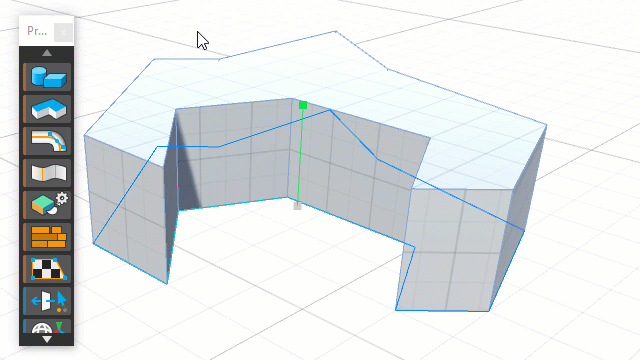
\includegraphics[width = 0.6\textwidth]{Planning report/images/probuilder-example.png}
    \caption{An example of the graphical interface of \textit{ProBuilder} \cite{unity-probuilder-procore}.}
    \label{fig:probuilder-editor}
\end{figure}

\begin{figure}[H]
\centering
\begin{subfigure}{.48\linewidth}
  \centering
  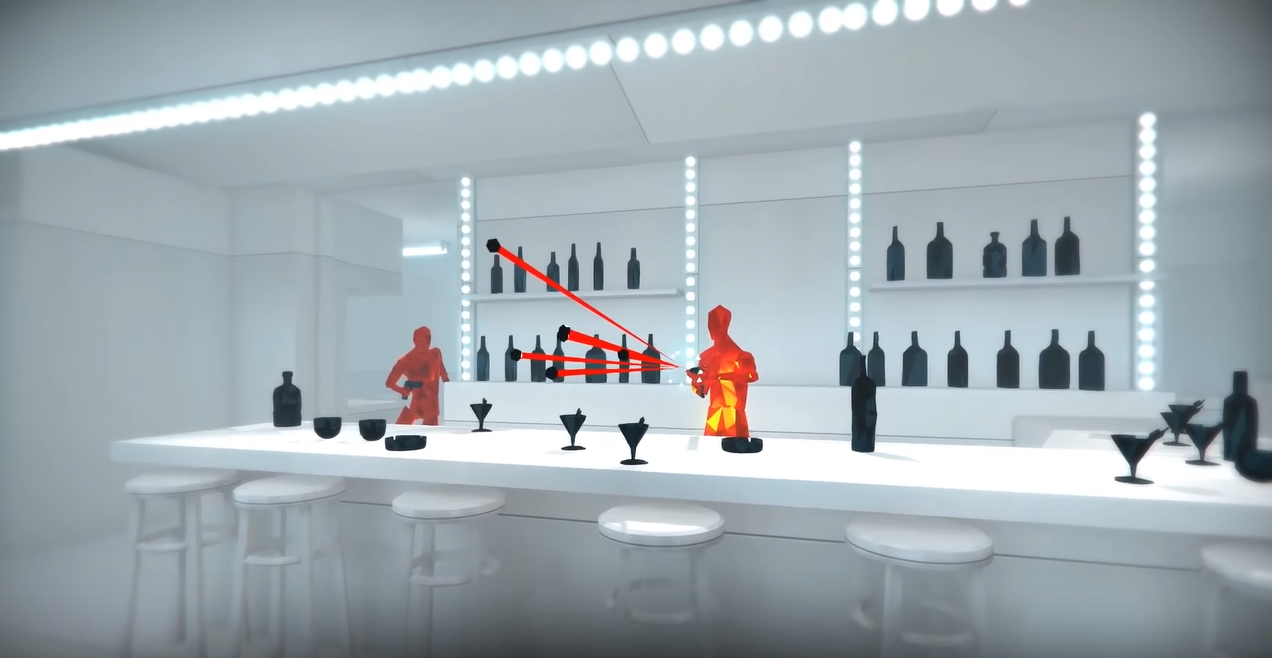
\includegraphics[width=1\linewidth]{Planning report/images/superhot-game.png}
  \caption{\textit{SUPERHOT}}
  \label{fig:superhot-game}
\end{subfigure}
~
\begin{subfigure}{.48\linewidth}
 \centering
  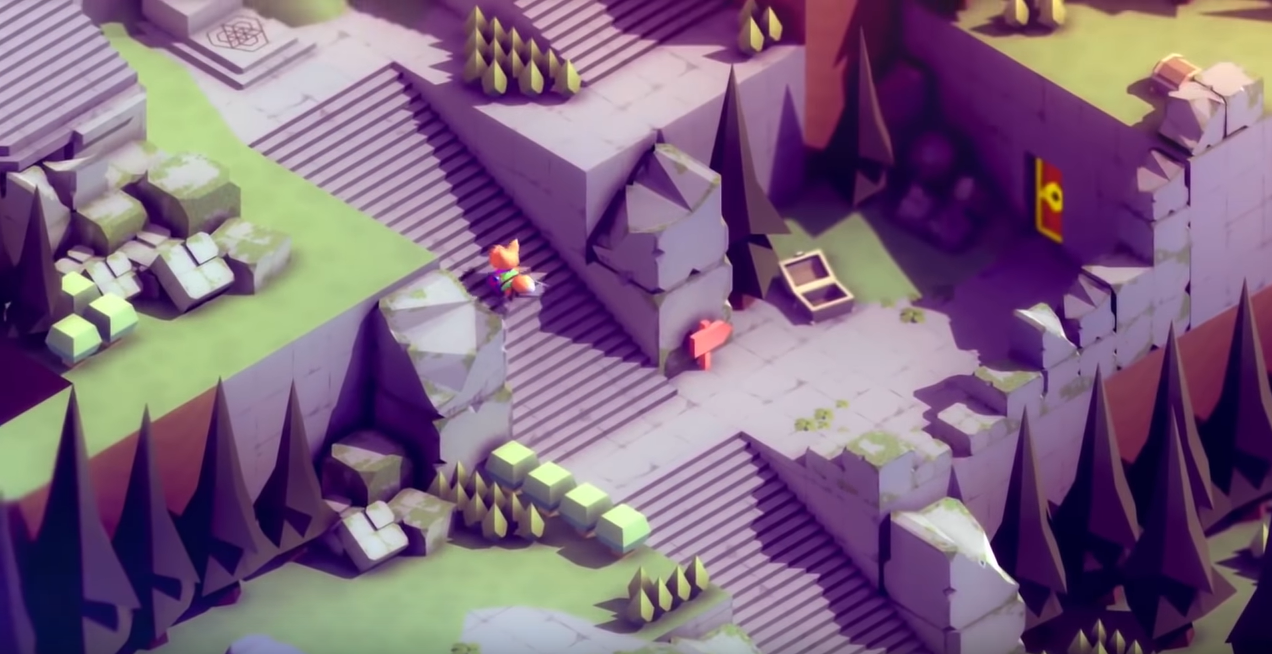
\includegraphics[width=1\linewidth]{Planning report/images/tunic-game.png}
  \caption{\textit{Tunic}}
  \label{fig:tunic-game}
\end{subfigure}
\caption{Screenshots of two games developed with \textit{ProBuilder}.}
\label{fig:probuilder-games}
\end{figure}

\subsubsection{Playmaker}
\textit{Playmaker} is a visual scripting tool and has the highest rating in the Unity Asset Store. It is a tool for creating behaviours in games without writing code. Behaviours are instead defined with state machines in a custom graphical interface in Unity. Two examples of games that utilize the tool are: \textit{Hearthstone} and \textit{Hollow Knight} \cite{unity-hutong-playmaker}.

\begin{figure}[H]
    \centering
    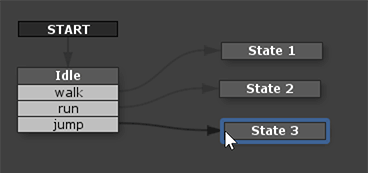
\includegraphics[width = 0.6\textwidth]{Planning report/images/playmaker-example.png}
    \caption{Screenshot of the graphical interface of \textit{Playmaker}.}
    \label{fig:playmaker-editor}
\end{figure}

\begin{figure}[H]
\centering
\begin{subfigure}{.48\linewidth}
  \centering
  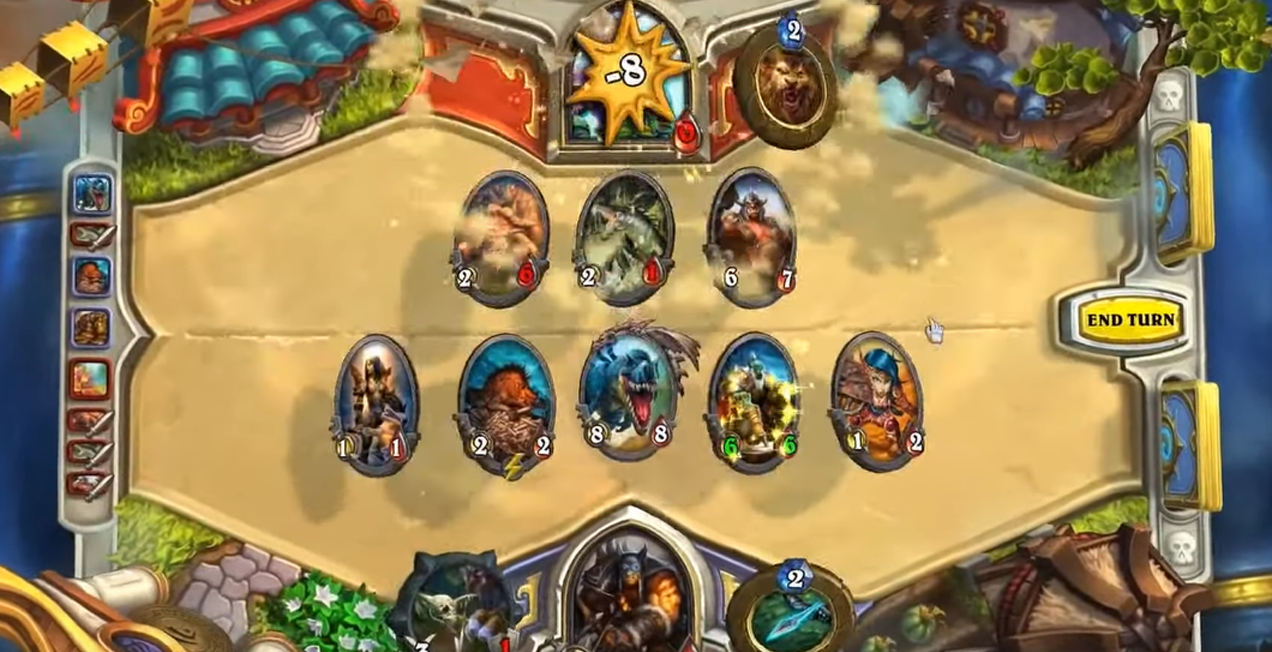
\includegraphics[width=1\linewidth]{Planning report/images/hearthstone-game.png}
  \caption{\textit{Hearthstone}}
  \label{fig:hearthstone-game}
\end{subfigure}
~
\begin{subfigure}{.48\linewidth}
  \centering
  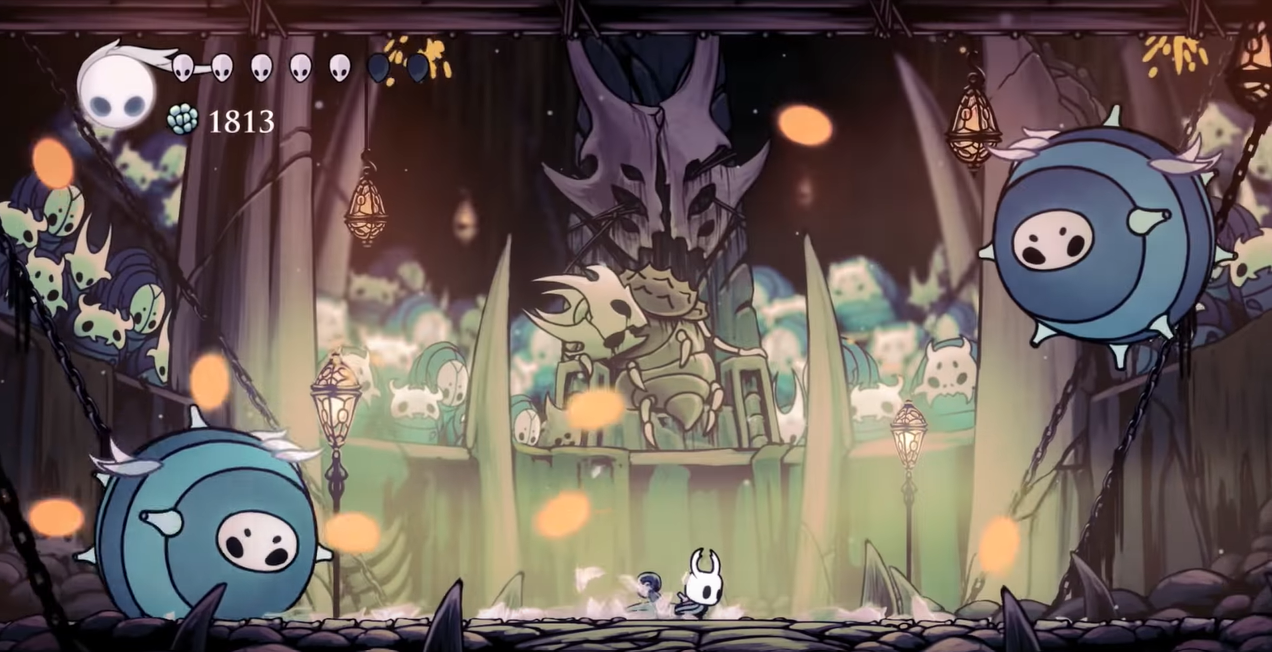
\includegraphics[width=1\linewidth]{Planning report/images/hollow_knight-game.png}
  \caption{\textit{Hollow Knight}}
  \label{fig:hollow-knight-game}
\end{subfigure}
\caption{Screenshots of two games developed with \textit{Playmaker}.}
\label{fig:playmaker-games}
\end{figure}

\subsubsection{Shader Forge}
\textit{Shader Forge} was released to the Unity Asset Store in 2011 \cite{unity-shadow-forge-forum} but has since then been removed. It is, however, still available on GitHub as an open-source repository \cite{unity-shadow-forge-github}. It is a tool for creating shaders without writing any code and has its own custom graphical interface based on nodes. The tool has been promoted by game developers known for games such as \textit{Dear Esther} and \textit{Knytt Underground} \cite{unity-shadow-forge}.

\begin{figure}[H]
    \centering
    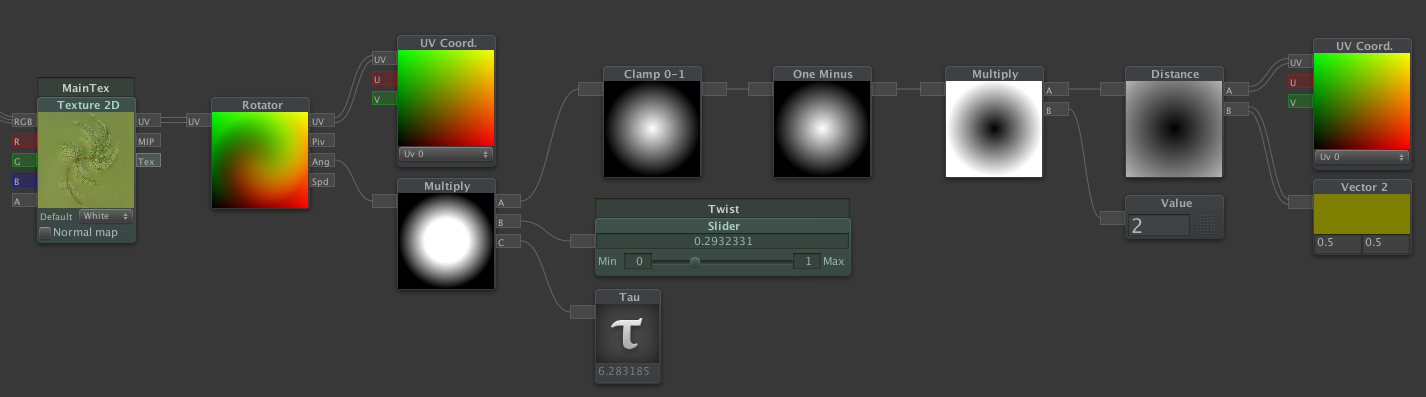
\includegraphics[width = \textwidth]{Planning report/images/unity-shader-forge.jpg}
    \caption{A screenshot of the graphical interface of \textit{Shader Forge} \cite{unity-shadow-forge-forum}.}
    \label{fig:shader-forge-editor}
\end{figure}